\pdfminorversion=4
\documentclass[aspectratio=169]{beamer}

\mode<presentation>
{
  \usetheme{default}
  \usecolortheme{default}
  \usefonttheme{default}
  \setbeamertemplate{navigation symbols}{}
  \setbeamertemplate{caption}[numbered]
  \setbeamertemplate{footline}[frame number]  % or "page number"
  \setbeamercolor{frametitle}{fg=white}
  \setbeamercolor{footline}{fg=black}
} 

\usepackage[english]{babel}
\usepackage[utf8x]{inputenc}
\usepackage{tikz}
\usepackage{courier}
\usepackage{array}
\usepackage{bold-extra}
\usepackage{minted}
\usepackage[thicklines]{cancel}
\usepackage{fancyvrb}

\xdefinecolor{dianablue}{rgb}{0.18,0.24,0.31}
\xdefinecolor{darkblue}{rgb}{0.1,0.1,0.7}
\xdefinecolor{darkgreen}{rgb}{0,0.5,0}
\xdefinecolor{darkgrey}{rgb}{0.35,0.35,0.35}
\xdefinecolor{darkorange}{rgb}{0.8,0.5,0}
\xdefinecolor{darkred}{rgb}{0.7,0,0}
\definecolor{darkgreen}{rgb}{0,0.6,0}
\definecolor{mauve}{rgb}{0.58,0,0.82}

\title[2019-11-07-chep-awkward]{Alexander and the Ragged, Jagged, \\ Nested, Indirected, Very Awkward Arrays}
\author{\underline{Jim Pivarski}, David Lange, Peter Elmer}
\institute{Princeton University -- IRIS-HEP}
\date{November 7, 2019}

\usetikzlibrary{shapes.callouts}

\begin{document}

\logo{\pgfputat{\pgfxy(0.11, 7.4)}{\pgfbox[right,base]{\tikz{\filldraw[fill=dianablue, draw=none] (0 cm, 0 cm) rectangle (50 cm, 1 cm);}\mbox{\hspace{-8 cm}
\includegraphics[height=1 cm]{princeton-logo-long.png}\hspace{0.1 cm}\raisebox{0.1 cm}{
\includegraphics[height=0.8 cm]{iris-hep-logo-long.png}}\hspace{0.1 cm}}}}}

\begin{frame}
  \titlepage

\vspace{-3.5 cm}
\hfill 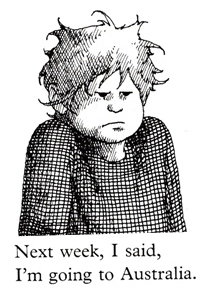
\includegraphics[height=4.5 cm]{alexander.png}
\vspace{-1 cm}
\end{frame}

\logo{\pgfputat{\pgfxy(0.11, 7.4)}{\pgfbox[right,base]{\tikz{\filldraw[fill=dianablue, draw=none] (0 cm, 0 cm) rectangle (50 cm, 1 cm);}\mbox{\hspace{-8 cm}
\includegraphics[height=1 cm]{princeton-logo.png}\hspace{0.1 cm}\raisebox{0.1 cm}{
\includegraphics[height=0.8 cm]{iris-hep-logo.png}}\hspace{0.1 cm}}}}}

% Uncomment these lines for an automatically generated outline.
%\begin{frame}{Outline}
%  \tableofcontents
%\end{frame}

% START START START START START START START START START START START START START

\begin{frame}{In a data analysis, physicists need\ldots}
\Large
\vspace{-0.5 cm}

\begin{columns}[t]
\column{0.5\linewidth}
\begin{center}
\textcolor{darkblue}{\LARGE rich data structures}
\end{center}

\vspace{-0.2 cm}
You can get that with C++ or Python, but C++ is verbose for analysis and Python is slow.

\column{0.5\linewidth}
\begin{uncoverenv}<2->
\begin{center}
\textcolor{darkblue}{\LARGE interactivity}
\end{center}

\vspace{-0.2 cm}
Data-oriented DSLs like NumPy and Pandas are convenient, but only for rectangular arrays of numbers.
\end{uncoverenv}
\end{columns}

\vspace{0.25 cm}
\begin{columns}
\column{0.5\linewidth}
\begin{uncoverenv}<3->
\begin{center}
\textcolor{darkblue}{\LARGE speed}
\end{center}

\vspace{-0.2 cm}
Results should pop up quickly enough that you don't lose your train of thought.
\end{uncoverenv}
\end{columns}
\end{frame}

\begin{frame}{Any data structure can be arranged as columnar arrays}
\begin{center}
\only<1>{\vspace{0.75 cm}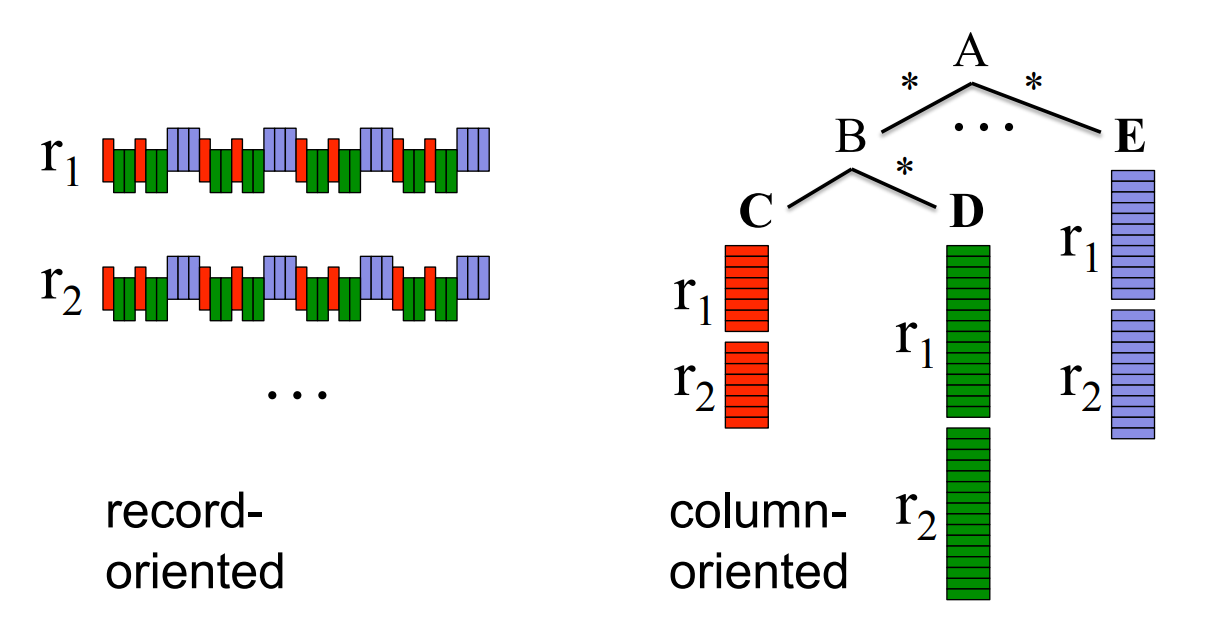
\includegraphics[width=0.8\linewidth]{google-dremel-fig1.png}}\only<2>{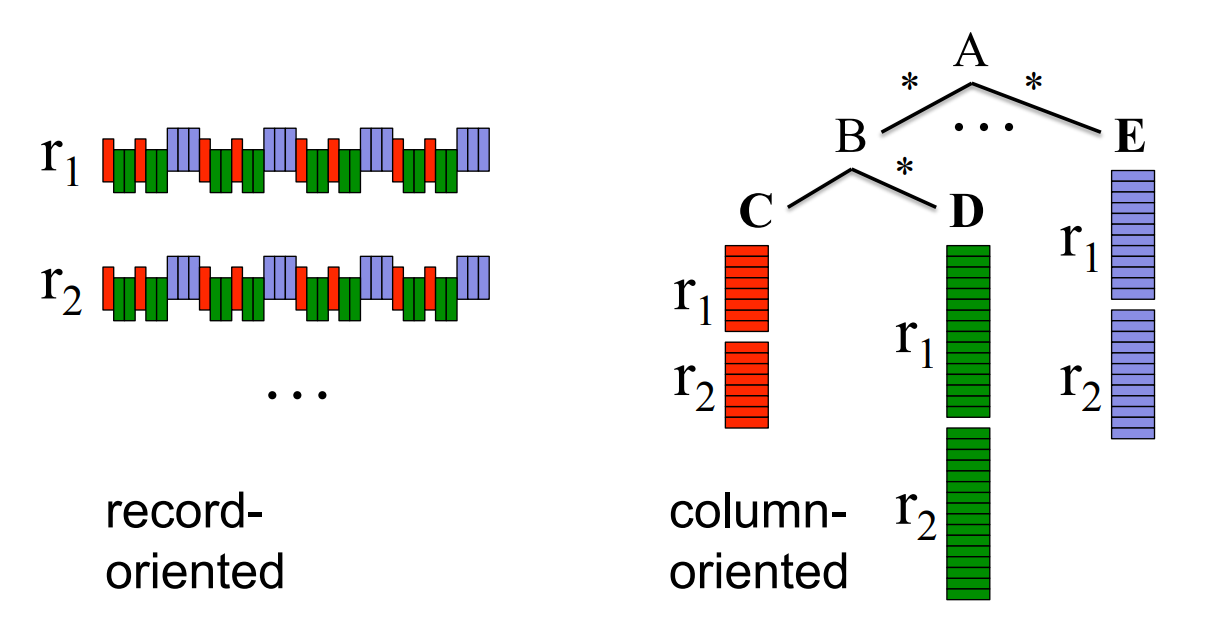
\includegraphics[width=0.55\linewidth]{google-dremel-fig1.png}}
\end{center}

\vspace{-0.25 cm}
\begin{uncoverenv}<2->
\begin{columns}
\column{1.08\linewidth}
\textcolor{darkblue}{Clickable links to prior art:}

\scriptsize
\begin{itemize}
\item \href{https://web.archive.org/web/19970225083621/http://root.cern.ch/root/HowtoWriteTree.html}{ROOT I/O with object splitting \textcolor{darkorange}{\bf (1997)}.}
\item \href{https://ai.google/research/pubs/pub36632}{M.\ Sergey et.\ al.\ (Google Dremel) {\it Proc. of the 36th Int'l Conf on Very Large Data Bases} \textcolor{darkorange}{\bf (2010)}, pp. 330--339.}
\item \href{https://dl.acm.org/citation.cfm?id=2814228.2814230}{T.\ Mattis et.\ al., ``Columnar Objects: Improving the Performance of Analytical Applications,'' in {\it ACM Int'l Symp.\ on New Ideas, New Paradigms, and Reflections on Programming and Software (Onward!),} \textcolor{darkorange}{\bf (2015)}, pp.\ 197--210.}
\item \href{https://parquet.apache.org}{Parquet file format \textcolor{darkorange}{\bf (2015)}}.
\item \href{https://arrow.apache.org}{Apache Arrow in-memory format \textcolor{darkorange}{\bf (2016)}}.
\item \href{https://zarr.readthedocs.io/en/stable/tutorial.html\#ragged-arrays}{Zarr data delivery system \textcolor{darkorange}{\bf (2015)}}.
\end{itemize}

\vspace{-1 cm}
\mbox{\hspace{0.5\linewidth}\begin{minipage}{0.5\linewidth}
\begin{itemize}
\item \href{https://xnd.io}{XND vectorized math library \textcolor{darkorange}{\bf (2018)}}.
\item \href{https://www.tensorflow.org/guide/ragged_tensor}{TensorFlow RaggedTensor \textcolor{darkorange}{\bf (2018)}}.
\end{itemize}
\end{minipage}}
\end{columns}
\end{uncoverenv}
\end{frame}

\begin{frame}{Building columnar data structures from single-purpose parts}
\large
\vspace{0.25 cm}
\begin{center}
\only<1>{An array of variable-length arrays (``ragged'' or ``jagged'') can be built out of flattened contents and offsets specifying the beginning of each subarray.}\only<2>{Multiple levels of variable-length arrays (``doubly jagged'') can be built by using one jagged array as the content of the other.}\only<3>{Complex data structures can be built if you have enough columnar components, such as records with named fields, mixed data types, pointers, lazy loading\ldots}
\end{center}

\vspace{-0.25 cm}
\begin{columns}
\column{1.15\linewidth}
\only<1>{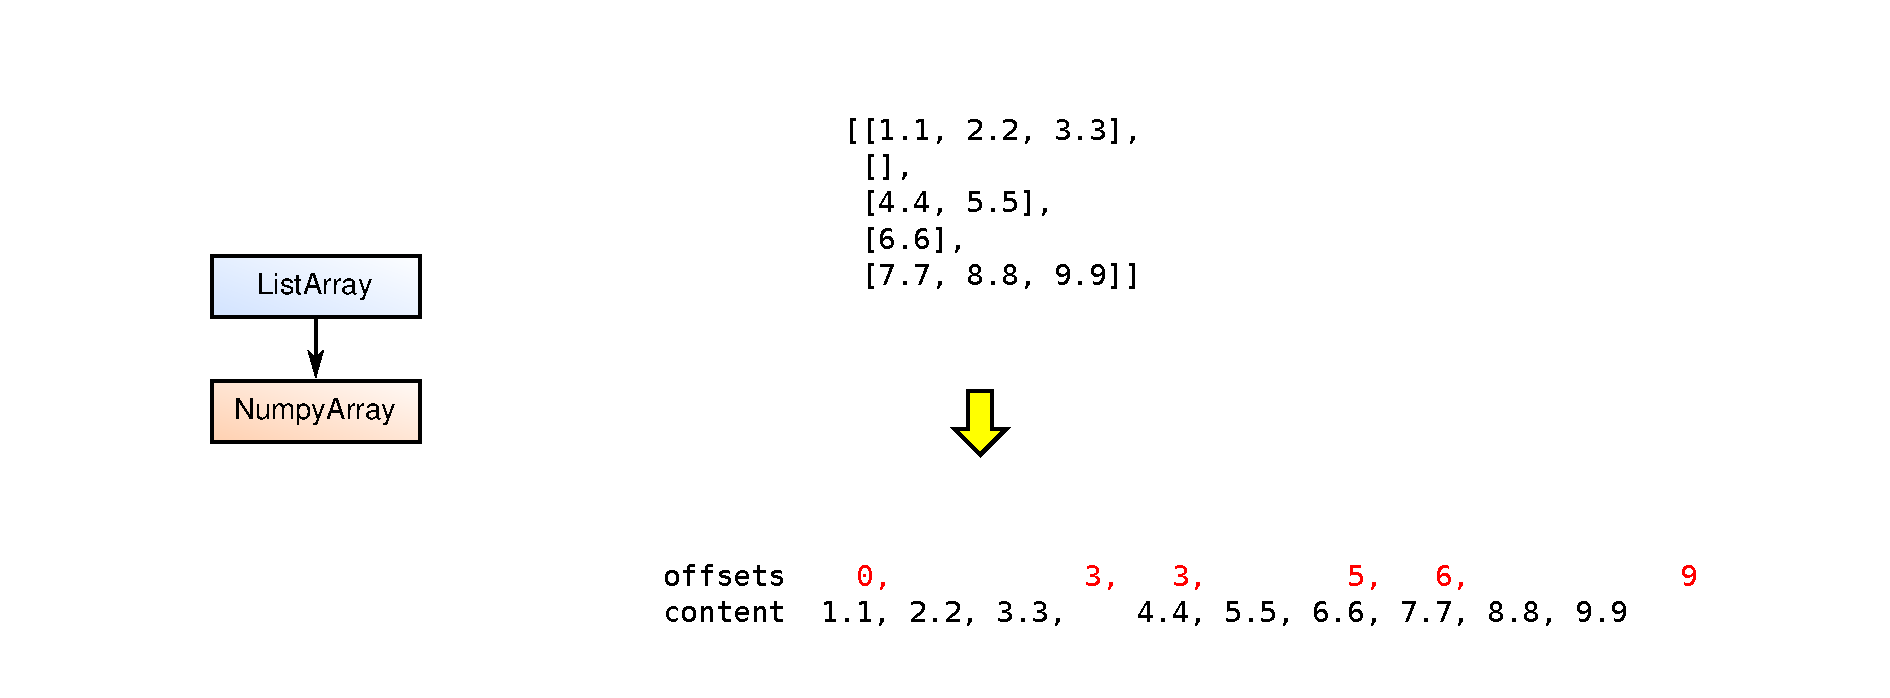
\includegraphics[width=\linewidth]{composable-1.pdf}}\only<2>{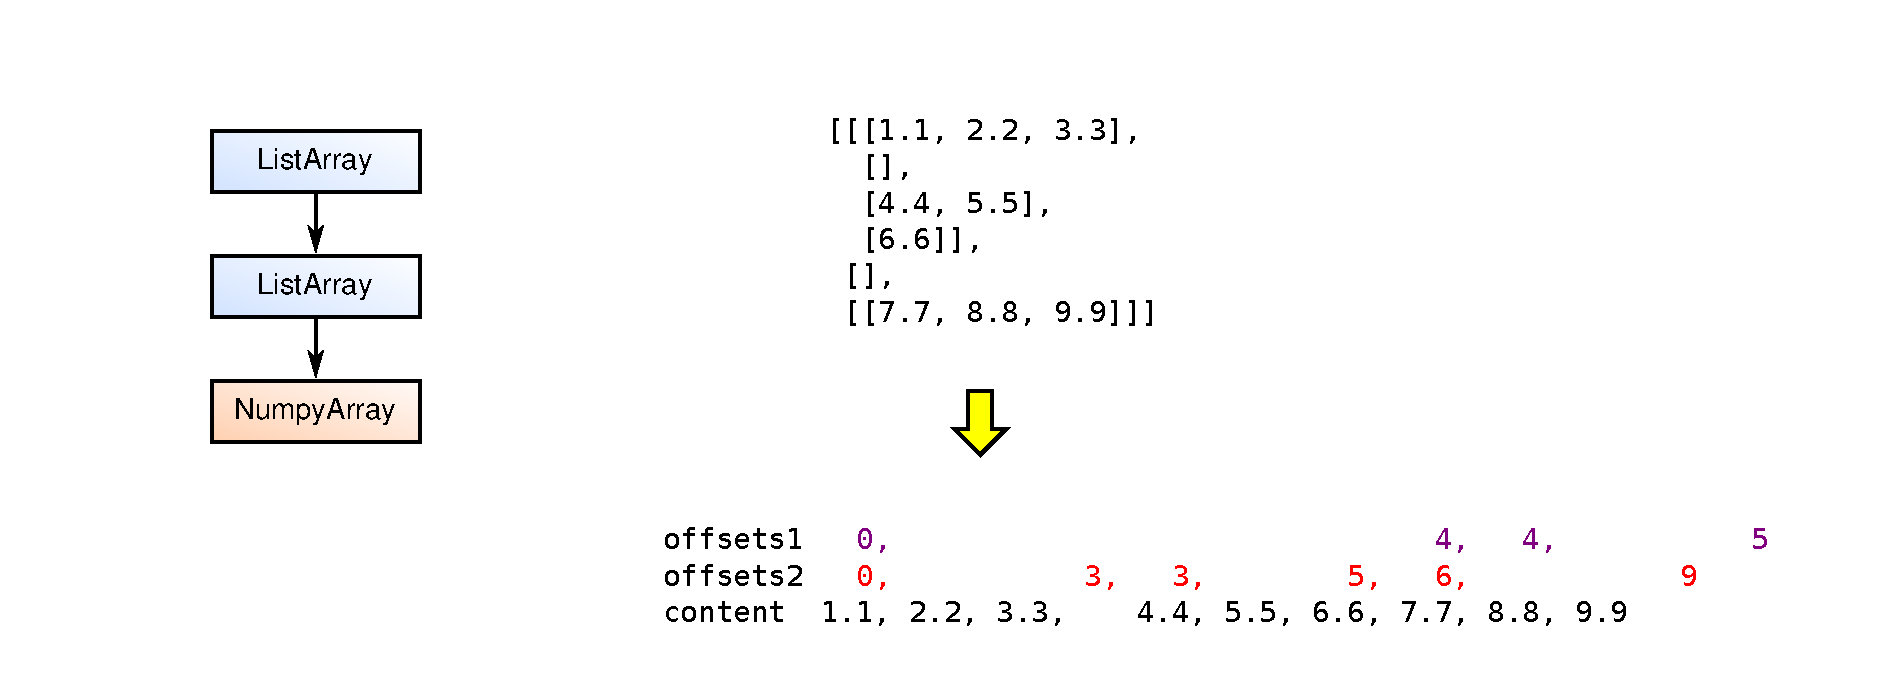
\includegraphics[width=\linewidth]{composable-2.pdf}}\only<3>{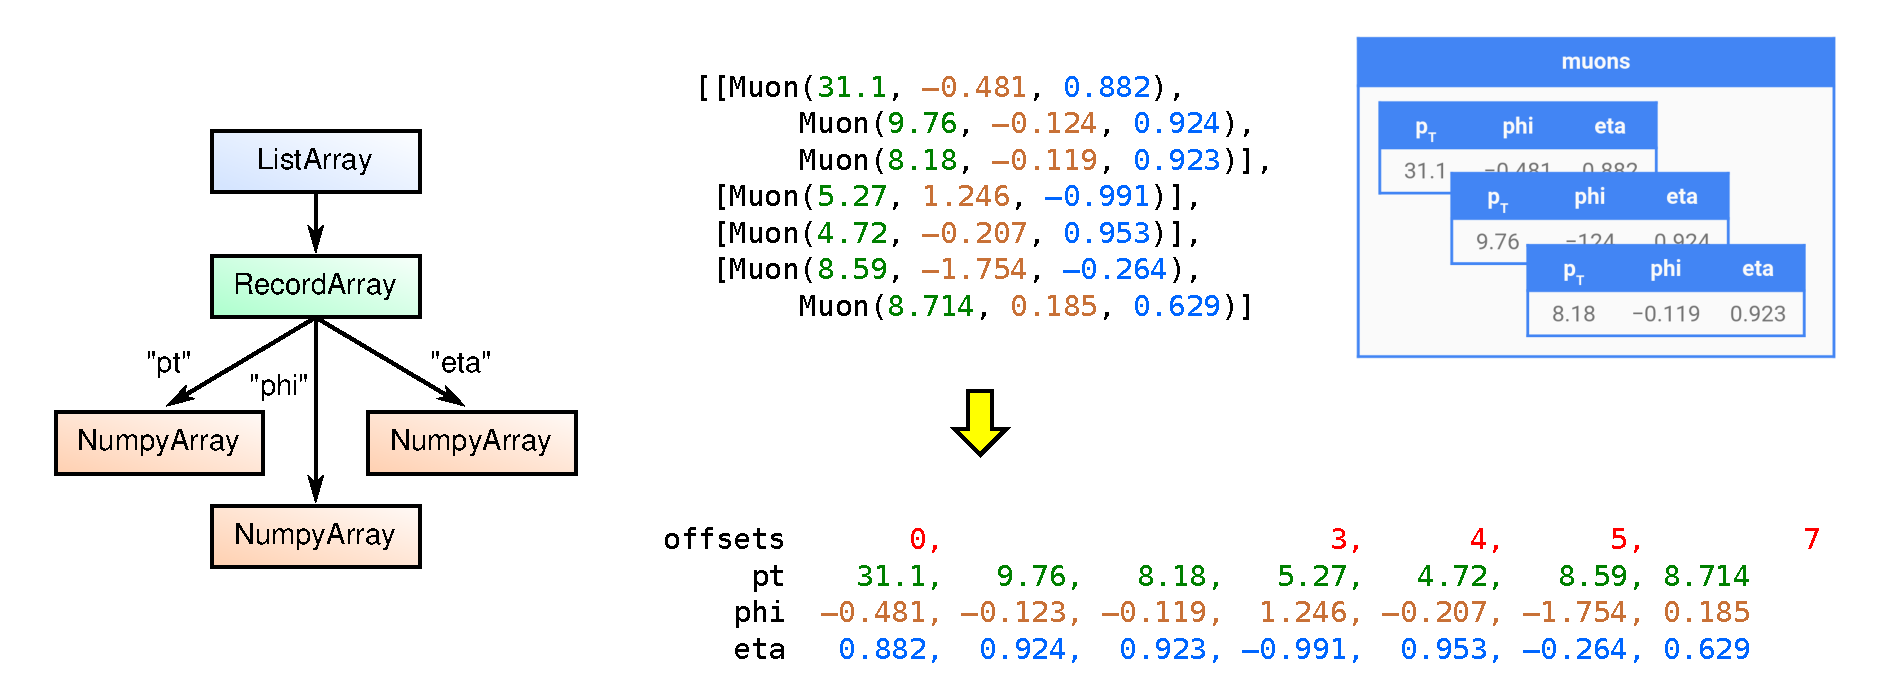
\includegraphics[width=\linewidth]{composable-3.pdf}}
\end{columns}
\end{frame}

\begin{frame}{\mbox{ }}
\vspace{0.5 cm}
\begin{center}

\includegraphics[width=0.5\linewidth]{awkward-logo.pdf}
\end{center}
\end{frame}

\begin{frame}{We now have 1 year of user feedback and maintainance experience}
\large
\vspace{0.5 cm}

\begin{columns}
\column{0.75\linewidth}
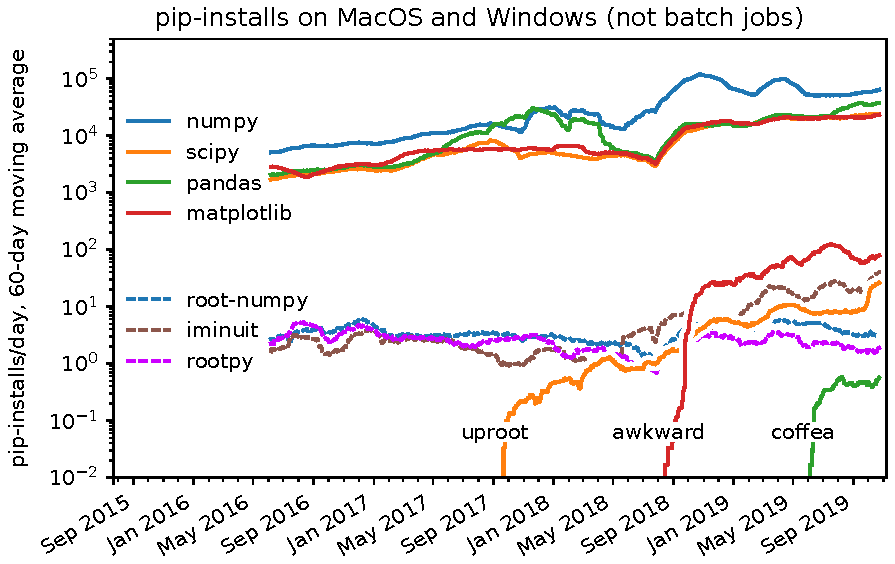
\includegraphics[width=\linewidth]{pip-timeline.pdf}

\vspace{0.1 cm}
\centering \textcolor{darkblue}{\fbox{awkward has 100 downloads/day, 2 issues/week}}

\column{0.3\linewidth}
\hfill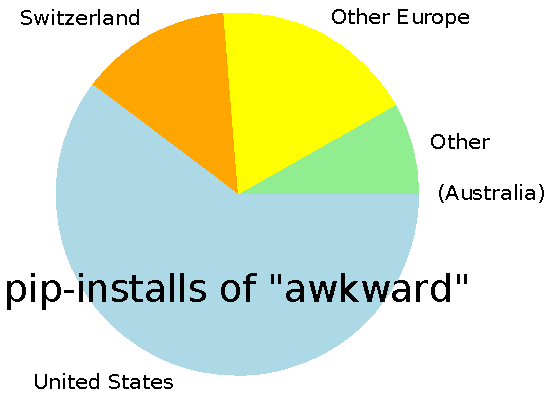
\includegraphics[width=0.8\linewidth]{pip-country-awkward.pdf}

\vspace{0.2 cm}
\hspace{-0.25 cm}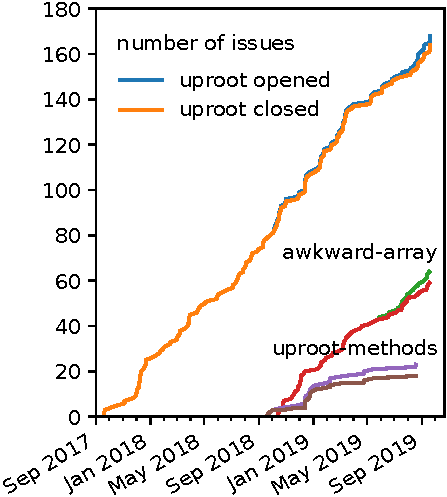
\includegraphics[width=\linewidth]{uproot-issues.pdf}
\end{columns}
\end{frame}

\begin{frame}{What I've learned}
\large
\vspace{0.5 cm}
\begin{block}{\Large From feedback and tutorials:}
\vspace{0.2 cm}
The interface needs to be simpler: a single \mintinline{python}{awkward.Array} class to hide the \mintinline{python}{ListArray} $\to$ \mintinline{python}{RecordArray} $\to$ \mintinline{python}{NumpyArrays} structure.

\vspace{0.2 cm}
Separate structural operations (e.g.\ cross-join) from physics (e.g.\ cross-product).
\end{block}

\vspace{0.5 cm}
\begin{uncoverenv}<2->
\begin{block}{\Large From maintenance:}
\vspace{0.2 cm}
Current implementation is entirely written in Python/Numpy.

\vspace{0.2 cm}
For better flexibility, robustness, and uniformity, and in a few cases, speed, it should be rewritten in C++.
\end{block}
\end{uncoverenv}
\end{frame}

\begin{frame}{New architecture}
\large
\vspace{0.5 cm}
\begin{columns}
\column{0.5\linewidth}
\vspace{-0.2 cm}

\textcolor{darkblue}{Layer 1:} Python user interface: a single \mintinline{python}{awkward.Array} class.
\vspace{\baselineskip}

\vspace{0.18 cm}
\begin{uncoverenv}<2->
\textcolor{darkblue}{Layer 2:} Structural classes in Python

(e.g.\ \mintinline{python}{ListArray}/\mintinline{python}{RecordArray}).
\end{uncoverenv}
\vspace{\baselineskip}

\vspace{0.18 cm}
\begin{uncoverenv}<3->
\textcolor{darkblue}{Layer 3:} Array allocation and ownership; reference counting. Two languages: C++ and Numba (compiled Python).
\end{uncoverenv}
\vspace{\baselineskip}

\vspace{0.18 cm}
\begin{uncoverenv}<4->
\textcolor{darkblue}{Layer 4:} Implementations, where we write \mintinline{python}{for} loops. The only layer that needs to be optimized for speed.
\end{uncoverenv}

\column{0.5\linewidth}
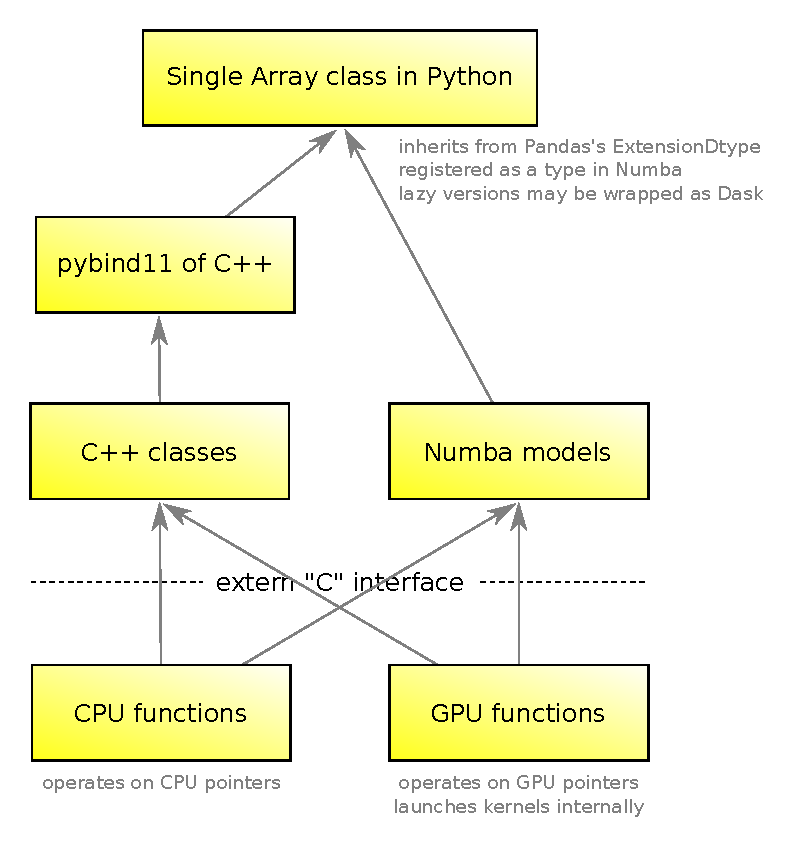
\includegraphics[width=\linewidth]{awkward-1-0-layers.pdf}
\end{columns}
\end{frame}

\begin{frame}[fragile]{First benefit: greater generality}
\large
\vspace{0.35 cm}
\hfill\mbox{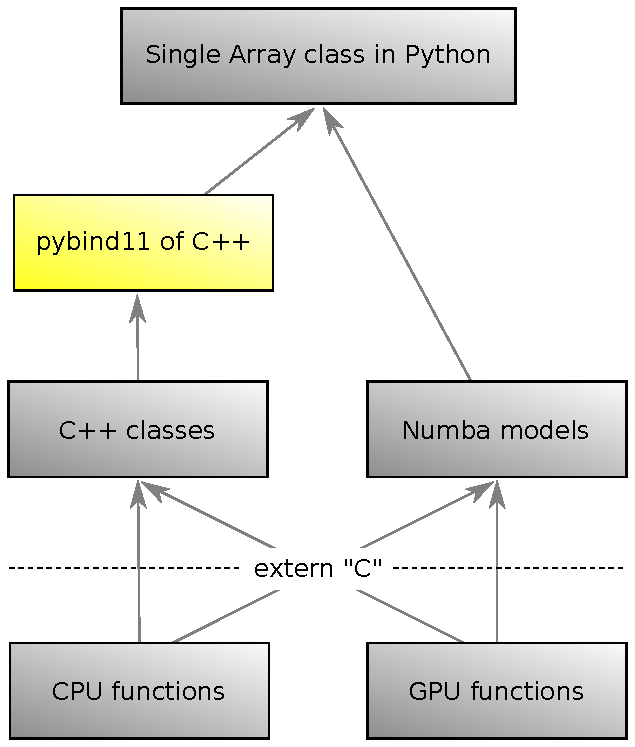
\includegraphics[height=4 cm]{awkward-1-0-layers-mini-pybind11.pdf}\hspace{-0.75 cm}}

\vspace{-4 cm}
\begin{columns}
\column{1.1\linewidth}
The current implementation has some hidden limitations, such as \\ slicing in more than two jagged dimensions.

\scriptsize
\vspace{0.1 cm}
\begin{minted}{python}
>>> import awkward    # awkward 0.x
>>> array = awkward.fromiter([[[0.0, 1.1, 2.2], [], [3.3, 4.4]],
...                           [[5.5]], [], [[6.6, 7.7, 8.8, 9.9]]])
>>> array[::-1, ::2, 1:].tolist()
\end{minted}
\begin{Verbatim}[commandchars=\\\{\}]
\textcolor{red}{NotImplementedError: this implementation cannot slice a JaggedArray}
                     \textcolor{red}{in more than two dimensions}
\end{Verbatim}

\large
\vspace{0.5 cm}
But the new implementation is based on \mintinline{c++}{for} loops and recursive procedures that can go arbitrarily deep.

\scriptsize
\vspace{0.1 cm}
\begin{minted}{python}
>>> import awkward1   # awkward 1.0
>>> array = awkward1.fromiter([[[0.0, 1.1, 2.2], [], [3.3, 4.4]],
...                            [[5.5]], [], [[6.6, 7.7, 8.8, 9.9]]])
>>> awkward1.tolist(array[::-1, ::2, 1:])
\end{minted}
\begin{Verbatim}[commandchars=\\\{\}]
\textcolor{red}{[[[7.7, 8.8, 9.9]], [], [[]], [[1.1, 2.2], [4.4]]]}
\end{Verbatim}

\vspace{5 cm}
\end{columns}
\end{frame}

\begin{frame}[fragile]{Full access in C++}
\large
\vspace{0.35 cm}
\hfill\mbox{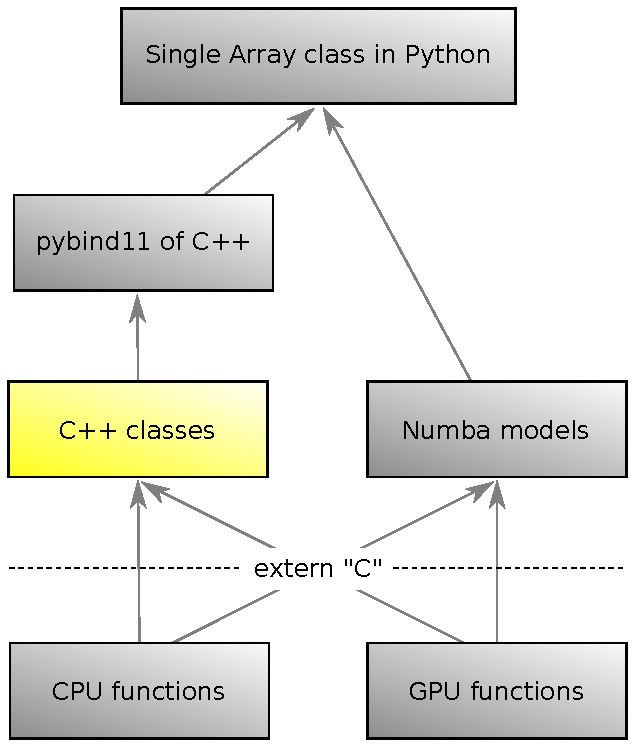
\includegraphics[height=4 cm]{awkward-1-0-layers-mini-cpp.pdf}\hspace{-0.75 cm}}

\vspace{-4 cm}
\begin{columns}
\column{1.1\linewidth}
Everything is available in C++ except the convenient syntax.

\scriptsize
\begin{minted}{c++}
namespace ak = awkward;
int main(int, char**) {
  std::vector<std::vector<std::vector<double>>> vector =
      {{{0.0, 1.1, 2.2}, {}, {3.3, 4.4}}, {{5.5}}, {},
       {{6.6, 7.7, 8.8, 9.9}}};

  ak::FillableArray builder(ak::FillableOptions(1024, 2.0));
  for (auto x : vector)
      builder.fill(x);
  std::shared_ptr<ak::Content> array = builder.snapshot();

  ak::Slice slice;
  slice.append(ak::SliceRange(ak::Slice::none(), ak::Slice::none(), -1));   // ::-1
  slice.append(ak::SliceRange(ak::Slice::none(), ak::Slice::none(), 2));    // ::2
  slice.append(ak::SliceRange(1, ak::Slice::none(), ak::Slice::none()));    // 1:

  if (array.get()->getitem(slice).get()->tojson(false, 1) !=
         "[[[7.7,8.8,9.9]],[],[[]],[[1.1,2.2],[4.4]]]")
      return -1;
  return 0;
}
\end{minted}

\vspace{5 cm}
\end{columns}
\end{frame}

\begin{frame}[fragile]{Full access in Numba}
\large
\vspace{0.35 cm}
\hfill\mbox{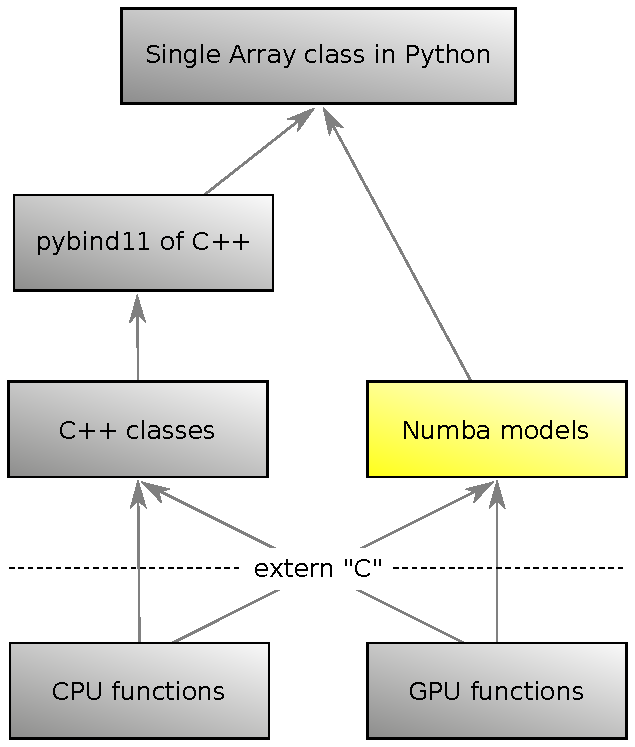
\includegraphics[height=4 cm]{awkward-1-0-layers-mini-numba.pdf}\hspace{-0.75 cm}}

\vspace{-4 cm}
\begin{columns}
\column{1.1\linewidth}
Similarly, everything is available in functions compiled by Numba.

\scriptsize
\vspace{0.1 cm}
\begin{minted}{python}
>>> import numba
>>>
>>> @numba.jit(nopython=True)
... def compileme(a):
...     return a[::-1, ::2, 1:]
... 
>>> compileme
\end{minted}
\begin{Verbatim}[commandchars=\\\{\}]
\textcolor{red}{CPUDispatcher(<function compileme at 0x7fd135e52ae8>)}
\end{Verbatim}
\begin{minted}{python}
>>> array = awkward1.fromiter([[[0.0, 1.1, 2.2], [], [3.3, 4.4]],
...                            [[5.5]], [], [[6.6, 7.7, 8.8, 9.9]]])
>>> awkward1.tolist(compileme(array))
\end{minted}
\begin{Verbatim}[commandchars=\\\{\}]
\textcolor{red}{[[[7.7, 8.8, 9.9]], [], [[]], [[1.1, 2.2], [4.4]]]}
\end{Verbatim}

\large
\vspace{0.25 cm}
\uncover<2->{Numba compiles a subset of Python; all data types must be known to the compiler.}

\vspace{0.25 cm}
\uncover<3->{Data analysts can start with pure Python and only accelerate the functions that need it.}

\vspace{5 cm}
\end{columns}
\end{frame}

\begin{frame}[fragile]{Single implementation}
\large
\vspace{0.35 cm}
\hfill\mbox{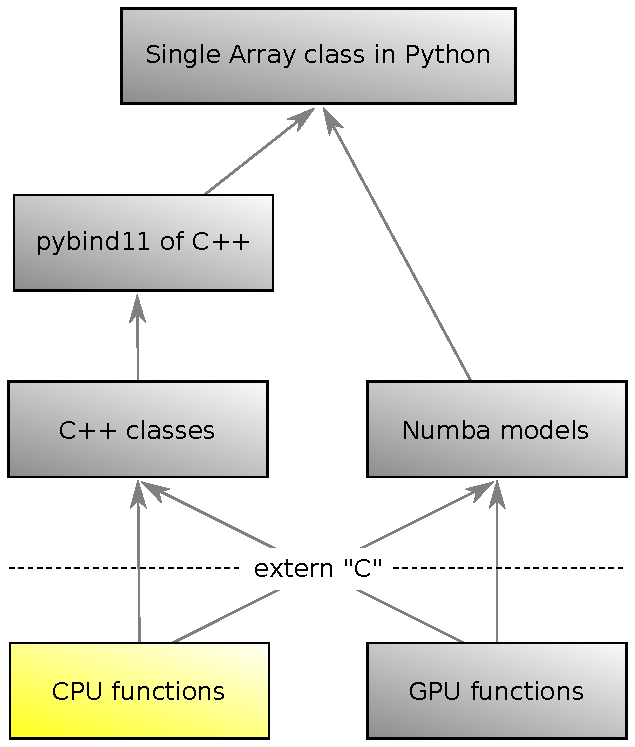
\includegraphics[height=4 cm]{awkward-1-0-layers-mini-cpu.pdf}\hspace{-0.75 cm}}

\vspace{-4 cm}
\begin{columns}
\column{1.1\linewidth}
All interfaces---Python, C++, Numba---share the same implementation, \\ a pure C library of functions on arrays.

\scriptsize
\begin{minted}{c++}
extern "C" {
  Error awkward_listarray32_getitem_next_at_64(int64_t* tocarry,
      const int32_t* fromstarts, const int32_t* fromstops,
      int64_t lenstarts, int64_t startsoffset, int64_t stopsoffset,
      int64_t at) {
    // This is only only layer with loops over array elements.
    for (int64_t i = 0;  i < lenstarts;  i++) {
      int64_t length = fromstops[stopsoffset + i] -
                       fromstarts[startsoffset + i];
      int64_t regular_at = at;
      if (regular_at < 0) {
        regular_at += length;
      }
      if (!(0 <= regular_at  &&  regular_at < length)) {
        return failure("index out of range", i, at);
      }
      tocarry[i] = fromstarts[startsoffset + i] + regular_at;
    }
    return success();
}
\end{minted}

\vspace{5 cm}
\end{columns}
\end{frame}

\begin{frame}[fragile]{Investigated toy languages with sets as a first-class concept}
\begin{center}
\fbox{\textcolor{blue}{\small \url{https://github.com/jpivarski/PartiQL}}}
\end{center}

\vspace{-0.25 cm}
\begin{columns}
\column{1.02\linewidth}
\scriptsize
\begin{Verbatim}[commandchars=\\\{\}]
\textcolor{gray}{# "For events with at least three leptons (electrons or muons) and a same-flavor}
\textcolor{gray}{# opposite-sign lepton pair, find the same-flavor opposite-sign lepton pair with a}
\textcolor{gray}{# mass closest to 91.2 GeV; make a histogram of the pT of the leading other lepton."}
\end{Verbatim}

\small
\vspace{-0.25 cm}
\begin{Verbatim}[commandchars=\\\{\}]
leptons = electrons \textcolor{darkgreen}{\textbf{union}} muons
\end{Verbatim}

\vspace{-0.45 cm}
\begin{Verbatim}[commandchars=\\\{\}]
\textcolor{darkgreen}{\textbf{cut}} \textcolor{blue}{count}(leptons) >= \textcolor{darkorange}{3} \textcolor{darkgreen}{\textbf{named}} \textcolor{darkorange}{"three_leptons"} \{
    Z = electrons \textcolor{darkgreen}{\textbf{as}} (lep1, lep2) \textcolor{darkgreen}{\textbf{union}} muons \textcolor{darkgreen}{\textbf{as}} (lep1, lep2)
            \textcolor{darkgreen}{\textbf{where}} lep1\textcolor{blue}{.charge} != lep2\textcolor{blue}{.charge}
            \textcolor{darkgreen}{\textbf{min by}} \textcolor{blue}{abs}(\textcolor{blue}{mass}(lep1, lep2) - \textcolor{darkorange}{91.2})
\end{Verbatim}

\vspace{-0.45 cm}
\begin{Verbatim}[commandchars=\\\{\}]
    third = leptons \textcolor{darkgreen}{\textbf{except}} [Z\textcolor{blue}{.lep1}, Z\textcolor{blue}{.lep2}] \textcolor{darkgreen}{\textbf{max by}} pt
    \textcolor{darkgreen}{\textbf{hist}} third.pt \textcolor{darkgreen}{\textbf{by}} \textcolor{blue}{regular}(\textcolor{darkorange}{100}, \textcolor{darkorange}{0}, \textcolor{darkorange}{250}) \textcolor{darkgreen}{\textbf{named}} \textcolor{darkorange}{"third_pt"}
\}
\end{Verbatim}

\large
\vspace{-0.45 cm}
\uncover<2->{\mbox{ }\hfill\rule{0.5\linewidth}{0.4 pt}\hfill\mbox{ }}

\vspace{0.2 cm}
\uncover<2->{To define operations on sets, such as \textcolor{darkgreen}{\tt\textbf{join}}, \textcolor{darkgreen}{\tt\textbf{cross}}, \textcolor{darkgreen}{\tt\textbf{union}}, and \textcolor{darkgreen}{\tt\textbf{except}}, we need what SQL calls a surrogate-key index, so this has been added as an optional \mintinline{c++}{Identity} array, passed through all operations in Awkward 1.0.}
\end{columns}
\end{frame}

\begin{frame}{PERFORMANCE PLOTS}

\end{frame}

\begin{frame}{Multi-paradigm arrays}
\large
\vspace{0.75 cm}
\textcolor{darkblue}{With a dataset in Awkward form (from TTrees, RNtuples, Arrow\ldots), we want to}

\vspace{0.25 cm}
\begin{itemize}\setlength{\itemsep}{0.25 cm}
\item perform vectorized operations with a Numpy-like syntax,
\item pass data to and from a C++ library,
\item enter a compiled Numba function to write fast for loops,
\item evaluate a declarative expression on sets of particles,
\end{itemize}

\vspace{0.25 cm}
\textcolor{darkblue}{interchangeably.}

\vspace{0.5 cm}
\begin{center}
\uncover<2->{\textcolor{darkorange}{\bf Awkward 1.0 is intended as a solid foundation for that future.}}
\end{center}
\end{frame}

\begin{frame}{When can I try it?}
\Large
\vspace{-0.25 cm}
\begin{center}
\fbox{\textcolor{blue}{\normalsize \url{https://github.com/scikit-hep/awkward-1.0}}}
\end{center}

\vspace{0.25 cm}
\begin{center}
\textcolor{darkblue}{Nowish:} it is in a testable state \textcolor{gray}{(for Coffea and thrill-seekers)}.

\vspace{0.75 cm}
Will be minimally usable for physics analysis in ``early 2020.''

\vspace{0.75 cm}
\end{center}

Start an {\normalsize \mintinline{python}{import awkward}} $\to$ {\normalsize \mintinline{python}{import awkward0}} \\
\phantom{Start an} {\normalsize \mintinline{python}{import awkward1}} $\to$ {\normalsize \mintinline{python}{import awkward}} transition by spring.
\end{frame}

\end{document}
